% Chapter 1

\chapter{Analisi} % Write in your own chapter title
\label{Chapter2}
\lhead{\emph{Analisi}}

\section{Le caratteristiche del MOS}
\label{sec:caratteristicheMos}

\subsection{Il modello semplificato del MOS}
\label{sec:sec_mos}

Dato che il circuito trattato in questo progetto è basato su tecnologia CMOS è doveroso iniziare con l'analisi del \textit{mattoncino base} che lo compone, ossia il transistor di tipo MOSFET.

\begin{figure}[hbt!]
	\centering
	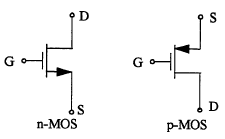
\includegraphics[width=0.5\textwidth]{figure/simboliMos.png}
	\caption{Simbolo NMOS (a sinistra) e PMOS (a destra)}
	\label{fig:simboliMos}
\end{figure}

Il modello semplificato introduce una \textit{tensione di soglia} $V_{th}$ e prevede che il dispositivo possa operare in tre zone di funzionamento, illustrate di seguito. Per semplicità consideriamo un NMOS; per il PMOS i segni di correnti e tensioni sono invertiti. 
\begin{itemize}
	\item \textit{Interdizione} - la $V_{GS}$ è sotto la soglia e non si è formato il canale, quindi la corrente di drain è nulla:
	\begin{equation}
	V_{GS} < V_{th_n} \qquad \Rightarrow \qquad I_D = 0 .
	\label{eq:eq_MOS_zonaInterdizione}
	\end{equation}
	
	\item \textit{Zona lineare} - $V_{GS}$ è sopra alla soglia e il canale si estende dal drain al source:
	\begin{equation}
	\begin{dcases}
	V_{GS} \geq V_{th_n} \\
	V_{DS}<V_{GS}-V_{th_n}
	\end{dcases}
	\qquad \Rightarrow \qquad I_{D} = \mu _{n} C^{'}_{ox} \frac{W}{L} \left[(V_{GS}-V_{th_n})V_{DS} - \frac{V_{DS}^2}{2} \right]
	\label{eq:eq_MOS_zonaLineare}
	\end{equation}
	se $V_{DS}$ è piccola il MOS si comporta come un resistore controllato da $V_{GS}$ (relazione lineare tra $V_{DS}$ e $I_D$):
	\begin{equation}
	I_{D} \simeq \mu _{n} C^{'}_{ox} \frac{W}{L} (V_{GS}-V_{th_n})V_{DS} .
	\label{eq:eq_MOS_zonaLineareApprox}
	\end{equation}
	
	\item \textit{saturazione} - $V_{GS}$ è sopra alla soglia e il canale presenta uno strozzamento in prossimità del drain; il MOS si comporta come un generatore di corrente $I_D$ costante, pilotato dalla tensione $V_{GS}$:
	\begin{equation}
	\begin{dcases}
	V_{GS} \geq V_{th_n} \\
	V_{DS} > V_{GS}-V_{th_n}
	\end{dcases}
	\qquad \Rightarrow \qquad 	I_{D} = \frac{1}{2} \mu _{n} C^{'}_{ox} \frac{W}{L} (V_{GS}-V_{th_n})^2 .
	\label{eq:eq_MOS_zonaSaturazione}
	\end{equation}
\end{itemize}

Le grandezze $\mu _n$ (\textit{mobilità dei portatori di carica}) e $C'_{ox}$ (\textit{capacità dell’ossido per unità di area tra gate e canale}) dipendono dalla tecnologia impiegata. Nel nostro caso (\textit{Microwind} $0.12 \ \mu m$) si ha:
\begin{itemize}
	\item NMOS: \quad $V_{th_n,0} = 0.40 \ V$; \ \quad $\mu _n = 600 \ \dfrac{cm^2}{V \cdot s}$
	\item PMOS: \quad $V_{th_p,0} = -0.45 \ V$; \quad $\mu _p = 200 \ \dfrac{cm^2}{V \cdot s}$
\end{itemize}
mentre per entrambi l'ossido ha spessore $t_{ox} = 2.0 \cdot 10^{-9} \ m$ e permittività elettrica relativa $\epsilon_{r_{Si0_2}} = 3.9$. Si ricava quindi:
\begin{equation}
C'_{ox} = \frac{\epsilon_0 \cdot \epsilon_r}{t_{ox}} = \dfrac{8.85 \cdot 10^{-12} \ [F/m] \cdot 3.9}{2.0 \cdot 10^{-9} \ [m]}\simeq 17.26 \cdot 10^{-3} \ \dfrac{F}{m^2}
\end{equation}

\subsection{La caratteristica reale del MOS}
\label{sec:sec_caratteristicaMOS}
Il modello del MOS mostrato nella sezione \ref{sec:sec_mos} è ben distante dalla realtà, perché si manifestano:
\begin{itemize}
	\item \textit{effetti di canale corto}, particolarmente visibili quando i transistor sono realizzati con la lunghezza minima disponibile per la tecnologia, come nel caso dei dispositivi digitali, in cui si vogliono minimizzare le dimensioni; ciò comporta la progressiva riduzione della velocità dei portatori di carica nel canale, diminuendo il fattore $\mu$ e quindi il guadagno;
	\item \textit{effetto body}, per il quale la $V_{th}$ diminuisce all'aumentare della tensione $V_{SB}$; nei dispositivi integrati spesso il source del MOS non è collegato al bulk (ovvero il substrato) e quindi $V_{SB} \neq 0 \Rightarrow \left | V_{th} \right | < \left | V_{th_0} \right | $ (con $V_{th_0}$ tensione di soglia per $V_{SB}=0$).
\end{itemize}

\subsection{Il modello \textit{level 3} di \textit{MicroWind}}
\label{sec:ilModelloDiMicrowind}
Il software \textit{MicroWind} fornisce un modello \textit{SPICE} del MOS di \textit{livello 3}, ben distante dalla caratteristica semplificata illustrata in sezione \ref{sec:sec_mos}. Di seguito, proponiamo un confronto tra i due modelli, facendo affidamento a curve caratteristiche ottenute mediante simulazione con \textit{LTspice}.

I grafici seguenti fanno riferimento ad un pMOS a dimensioni minime ($W = L = 0.12 \mu m$) generato da \textit{MicroWind}.

\begin{figure}[hbt!]
	\centering
	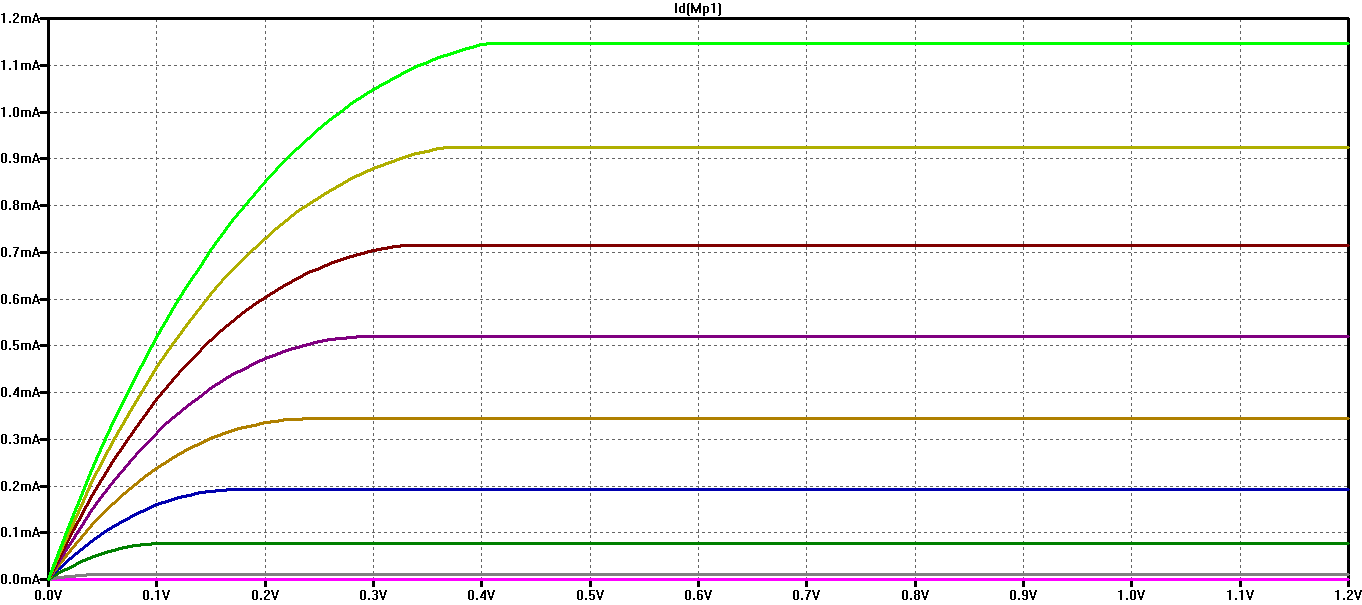
\includegraphics[width=1\textwidth]{figure/Sim_DCSweep_PMOS1_ConModelloAccurato(Chiaro).PNG}
	\caption{Curve caratteristiche di un pMOS - modello \textit{level 3} di \textit{MicroWind}.}
	\label{fig:curveCaratteristicheReali}
\end{figure}
Inizialmente abbiamo simulato il pMOS con il modello \textit{level 3} esattamente come generato da \textit{MicroWind}. Le curve nel piano $I_{DS}$ - $V_{DS}$ sono ottenute per incrementi costanti di $V_{GS}$ tra $0V$ e $V_{DD} = 1.2V$. Le correnti sono decisamente più basse rispetto a quanto atteso applicando le formule semplificate presentate in sezione \ref{sec:sec_mos}. Ad esempio, per $V_{GS} = 1.2V$, in saturazione si ha $I_D \approx 1.15mA$.

Per riportare il transistor ad un funzionamento più vicino al nostro modello quadratico approssimato, abbiamo provato ad ingannare il simulatore semplificando il modello \textit{SPICE}. In particolare dal listato di fig. \ref{fig:modelloMOSSpice} (per il pMOS, analogo per l'nMOS) abbiamo rimosso le prime due righe rosse, corrispondenti a parametri inesistenti nel nostro modello approssimato che comportano una notevole degradazione delle prestazioni dei transistor.

\begin{figure}[hbt!]
	\centering
	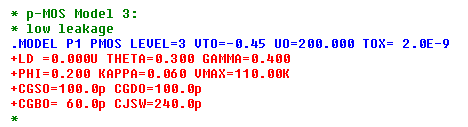
\includegraphics{figure/Cir_Snapshot_ModelloDelPMOSDiMicrowind.png}
	\caption{Modello \textit{SPICE} del pMOS fornito da \textit{MicroWind}.}
	\label{fig:modelloMOSSpice}
\end{figure}

Nelle nuove curve caratteristiche, per $V_{GS} = 1.2V$, in saturazione si ha $I_D \approx 2.9mA$.
Il risultato è aderente con quanto atteso applicando le formule semplificate, tuttavia non ha alcuna rilevanza pratica.

\begin{figure}[hbt!]
	\centering
	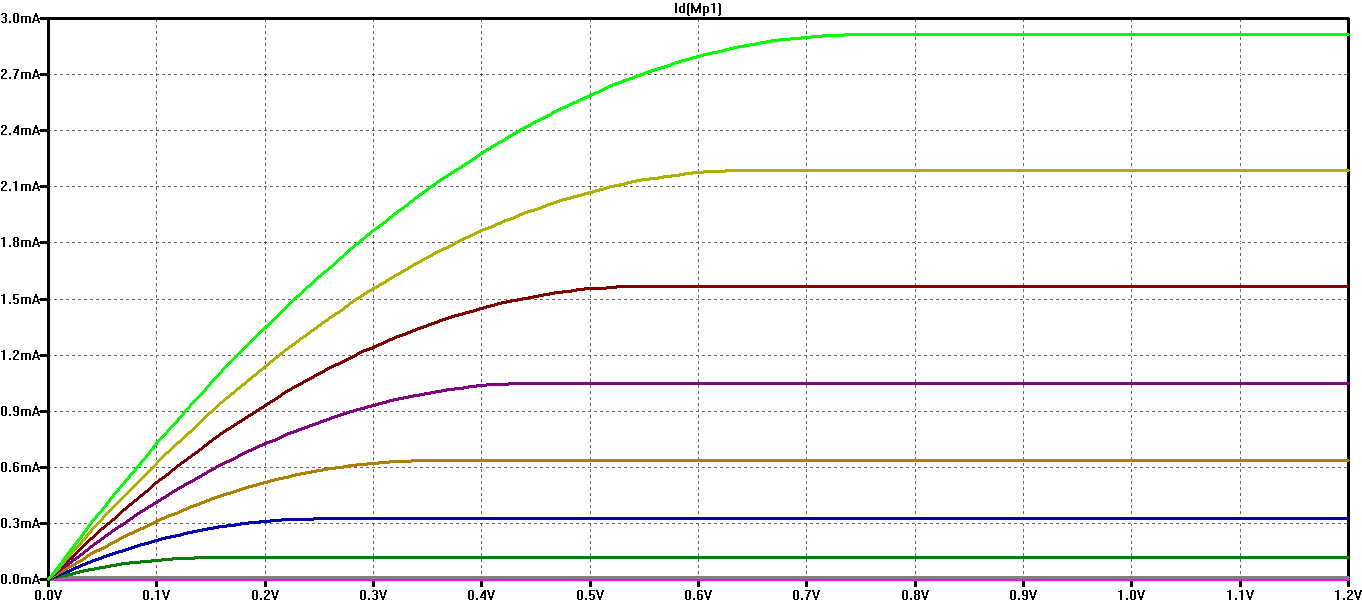
\includegraphics[width=1\textwidth]{figure/Sim_DCSweep_PMOS1_ModelloSemplificato(Chiaro).PNG}
	\caption{Curve caratteristiche di un pMOS - modello semplificato.}
	\label{fig:curveCaratteristicheSemplificate}
\end{figure}


\section{Funzionamento dinamico dei circuiti CMOS}
\label{sec:funzionamentoDinamicoCMOS}

Per valutare le prestazioni dinamiche della tecnologia CMOS, consideriamo come caso di studio un inverter con carico capacitivo ed effettuiamo un'analisi temporale fornendo in ingresso un'onda quadra.

\begin{figure}[hbt!]
	\centering
	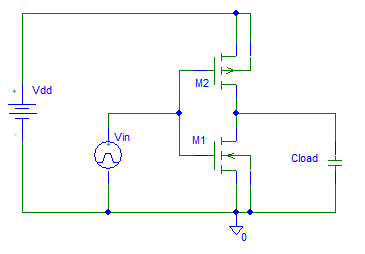
\includegraphics[width=0.5\textwidth]{figure/Sch_InverterCMOS.PNG}
	\caption{Inverter CMOS con capacità di carico.}
	\label{fig:fig_sch_inverterCMOS}
\end{figure}

\begin{figure}[hbt!]
	\centering
	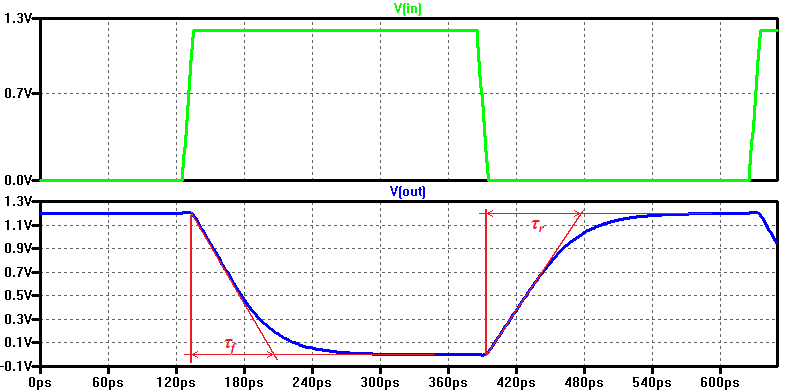
\includegraphics[width=1\textwidth]{figure/Sim_InverterCMOS(chiaro)WithNotes.png}
	\caption{Simulazione temporale di un inverter CMOS con capacità di carico.}
	\label{fig:fig_sim_inverterCMOS}
\end{figure}

Consideriamo un fronte di discesa della tensione d'uscita: in questo caso il condensatore, precedentemente caricato a $V_{DD}$ viene scaricato dal nMOS che funziona inizialmente in regime di saturazione ($V_{DS}>V_{GS}-V{th_n}$) per poi concludere la scarica in zona lineare. 

\begin{figure}[hbt!]
	\centering
	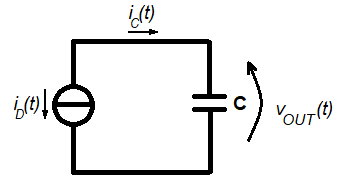
\includegraphics[width=0.4\textwidth]{figure/Sch_scaricaC.png}
	\caption{circuito equivalente per la scarica della capacità.}
	\label{fig:fig_sch_scaricaC}
\end{figure}

Questa situazione è schematizzata in figura \ref{fig:fig_sch_scaricaC}. La corrente $i_D(t) = - i_C(t)$ è quella che scorre nel canale del nMOS scaricando il condensatore. Si ha che:
\begin{equation}
i_C(t) = C \frac{d}{dt}v_{OUT}(t)
\label{eq:eq_condensatore}
\end{equation}
da cui, integrando tra $t_0$ e $t$, si ottiene l'evoluzione temporale di $v_{OUT}(t)$ a partire dalla condizione iniziale $v_{OUT}(t_0)$:
\begin{equation}
\int_{t_0}^{t} i_C(\xi)\, d\xi = C \int_{t_0}^{t} \frac{d}{d\xi}v_{OUT}(\xi)\, d\xi
\label{eq:eq_condensatoreIntegrata}
\end{equation}
ovvero, calcolando l'integrale a secondo membro e riordinando i termini:
\begin{equation}
v_{OUT}(t) - v_{OUT}(t_0) = \frac{1}{C}\int_{t_0}^{t} i_C(\xi)\, d\xi
\label{eq:eq_condensatoreSoluzione}
\end{equation}
Un'approssimazione valida per semplificare l'analisi si ottiene supponendo che il transistor operi solo in saturazione; esso si comporta quindi come un generatore di corrente costante e $i_C(t) = - i_D(t) = - I_D$; in tal caso l'integrale a secondo membro diventa una retta in $t$ e la scarica di $C$ ha un andamento lineare:

\begin{equation}
v_{OUT}(t) - v_{OUT}(t_0) \approx - \frac{1}{C}\int_{t_0}^{t} I_D \, d\xi = - \frac{I_D}{C}(t - t_0)
\label{eq:eq_condensatoreSoluzioneLineare}
\end{equation}

Questa formula, chiaramente, ha senso fisico finché $0 < V_{out}(t) < V_{DD}$, ovvero per i $t$ che soddisfano questo vincolo. Scegliendo un istante di tempo $t_1 > t_0$, si ha:
\begin{equation}
\Delta V = \left | v_{OUT}(t_1) - v_{OUT}(t_0) \right | \approx \frac{\left | I_D \right | }{C}(t_1 - t_0)
\label{eq:eq_condesatoreLineare}
\end{equation}

Nel caso del fronte di salita conduce il pMOS e si possono fare considerazioni analoghe; la \ref{eq:eq_condesatoreLineare} resta valida grazie agli operatori di valore assoluto.

Ai fini progettuali, in riferimento ai fronti di salita e discesa siamo interessati al tempo necessario per passare dal livello logico basso ($0V$) a quello alto  ($+V_{DD}$) e viceversa. Nel caso di fronte di discesa, iniziamo l'analisi con $C$ carico a $v_{OUT}(t_0) = V_{DD}$ e scegliamo $t_1 \ t.c. \ v_{OUT}(t_1) = 0$; facciamo il viceversa con il fronte di salita. Otteniamo così una comoda formula approssimata, valida in entrambi i casi:
\begin{equation}
\Delta V = \frac{\tau \left | I_D \right |}{C} \qquad \Leftrightarrow \qquad \left | I_D \right | = C \frac{\Delta V}{\tau}
\label{eq:eq_condensatoreLineareFinale}
\end{equation}
dove $\Delta V = V_{DD}$ è (in modulo) il "salto" di tensione da compiere e $\tau := t_1 - t_0$ è una stima del tempo di salita/discesa, ovvero il tempo di carica/scarica (lineare) della capacità $C = C_{load}$.

La validità di questa formula è discutibile: la stima del tempo di discesa è ottimistica ma è comunque utilizzabile come riferimento grossolano ai fini progettuali. Infatti, unendo questo risultato con l'equazione \ref{eq:eq_MOS_zonaSaturazione} (corrente di drain del MOS in saturazione) si ottiene una formula di progetto approssimata per determinare il rapporto d'aspetto necessario per avere i desiderati tempi di salita e discesa:

\begin{equation}
\frac{W}{L} =
\begin{dcases}
\frac{2 \ C_{load} \ V_{DD}}{\tau \mu _{n} C^{'}_{ox} (V_{DD}-V_{thn})^2} \quad nMOS\\
\frac{2\ C_{load} \ V_{DD}}{\tau \mu _{p} C^{'}_{ox} (V_{DD}-|V_{thp}|)^2} \quad pMOS
\end{dcases}
\label{eq:formulaRapportoAspetto}
\end{equation}

Una rappresentazione della carica/scarica lineare confrontata con l'andamento reale è visibile in figura \ref{fig:fig_sim_inverterCMOS}.

\section{Il Full Adder TSPC}
\label{sec:sec_fullAdder}

Analizziamo ora il circuito full adder TSPC presentato da Yuan e Svensson in \cite{yuan1989high}. Lo schema è mostrato in fig. \ref{fig:fig_schemaDaArticolo}.

\begin{figure}[hbt!]
	\centering
	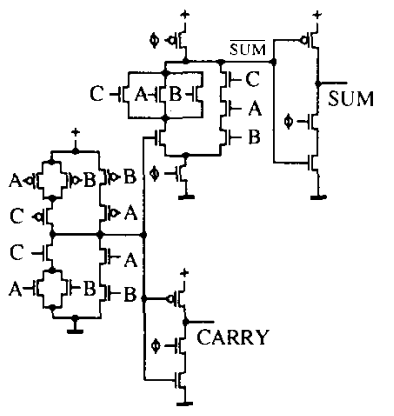
\includegraphics[width=0.5\textwidth]{figure/SchemaFullAdderTSPC_DaArticolo.PNG}
	\caption{TSPC full adder.}
	\label{fig:fig_schemaDaArticolo}
\end{figure}

La tecnica TSPC (\textit{True single phase clock}) permette di ottimizzare le performance di circuiti CMOS, soprattutto in termini di frequenza operativa. Tale risultato è raggiunto mediante la temporizzazione del funzionamento dei circuiti CMOS e più precisamente con l'aggiunta di un segnale di clock che, nel caso del circuito in esame, identifica due sole fasi in cui può trovarsi a lavorare quest'ultimo:

\begin{itemize}
	\item \textit{Fase di precarica}: il segnale di clock $\Phi$ è a livello logico basso, per cui i MOS di tipo \textit{p} pilotati da $\Phi$ si trovano in conduzione, mentre quelli di tipo \textit{n} sono in interdizione. Facendo riferimento allo schema di fig.  \ref{fig:fig_schemaDaArticolo} ciò implica che durante questo semiperiodo del segnale di clock il segnale \textit{!SUM} vada a livello alto, mentre i segnali \textit{SUM} e \textit{CARRY}, che tra l'altro sono i segnali di uscita, mantengano il valore cui si trovavano all'inizio del semiperiodo. 
	\item \textit{Fase di valutazione}: $\Phi$ è a livello alto, i pMOS da esso pilotati non conducono, a differenza degli nMOS. Nel circuito in esame questo implica che il valore logico dei segnali \textit{SUM} e \textit{CARRY} dipenda da tutti i restanti segnali, ovvero \textit{A},\textit{B}e \textit{C}, secondo la funzione logica tipica del sommatore full adder.
\end{itemize}

Valutiamo più precisamente cosa accade durante la fase di valutazione. Per farlo consideriamo la fig. \ref{fig:fig_schemaDaArticoloStadiCerchiati} dove sono stati evidenziati i quattro stadi che compongono il circuito.

\begin{figure}[hbt!]
	\centering
	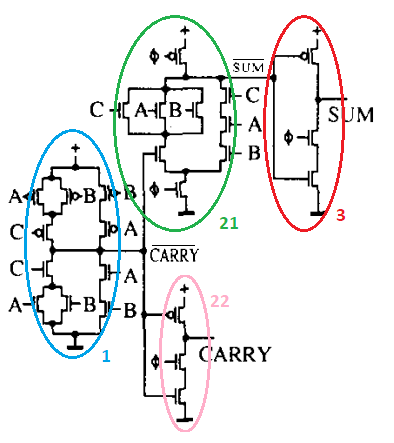
\includegraphics[width=0.5\textwidth]{figure/SchemaFullAdderTSPC_DaArticolo_ConStadiCerchiati.PNG}
	\caption{I quattro stadi che compongono il TSPC full adder.}
	\label{fig:fig_schemaDaArticoloStadiCerchiati}
\end{figure}

Per quanto riguarda il segnale \textit{SUM} lo stadio finale è il \textit{3}. La parte \textit{n} di questo stadio CMOS è costituita da due nMOS, uno pilotato dal segnale di temporizzazione $\Phi$ e uno dal segnale \textit{!SUM} generato dallo stadio precedente. \textit{!SUM} pilota anche l'unico transistor pMOS presente nella parte \textit{p}. Sull'uscita di questo stadio si ipotizza essere presente una capacità di carico pari a $100 fF$ come da specifiche. 

Il segnale \textit{!SUM} citato nel paragrafo precedente è a sua volta generato dallo stadio \textit{2.1}. La parte \textit{p} consiste in un solo pMOS pilotato da $\Phi$ che ha il compito di fornire in uscita un 1 logico durante la fase di precarica mentre delega alla parte \textit{n} la generazione di \textit{!SUM} durante la fase di valutazione. Quest'ultimo assumerà lo 0 logico solo se, durante la valutazione, è soddisfatta almeno una delle seguenti condizioni:

\begin{itemize}
	\item \textit{A}, \textit{B}, \textit{C} sono tutti alti contemporaneamente, cosicché i rispettivi nMOS possano condurre e creare così un percorso per la corrente dal nodo \textit{!SUM} a massa;
	\item \textit{!CARRY} è alto e almeno uno tra \textit{A}, \textit{B}, o \textit{C} è alto, per lo stesso motivo del punto precedente.
\end{itemize}

Lo stadio \textit{2.2} genera il segnale d'uscita \textit{CARRY} ed è del tutto analogo allo stadio \textit{3}.

Infine lo stadio \textit{1} si occupa di determinare il valore del segnale \textit{!CARRY}. La sua analisi è simile a quella dello stadio \textit{2.1}, sebbene questa volta non vi sia alcun transistor pilotato dal segnale di temporizzazione. \textit{!CARRY} assume livello logico basso quando si crea un percorso per la corrente tra il nodo di uscita e massa, cioè quando \textit{A} e \textit{B} sono alti o uno dei due è alto assieme a \textit{C}, cosicché i canali dei rispettivi nMOS sono presenti e il percorso si può così creare. Discorso duale vale per la parte \textit{p}: se \textit{A} e \textit{B} sono bassi, o uno dei due è basso assieme a \textit{C}, si forma un percorso di corrente tra l'alimentazione positiva e il nodo di uscita, ovvero \textit{!CARRY} assume livello logico alto.



